\documentclass[tikz,border=5mm]{standalone}

\begin{document}

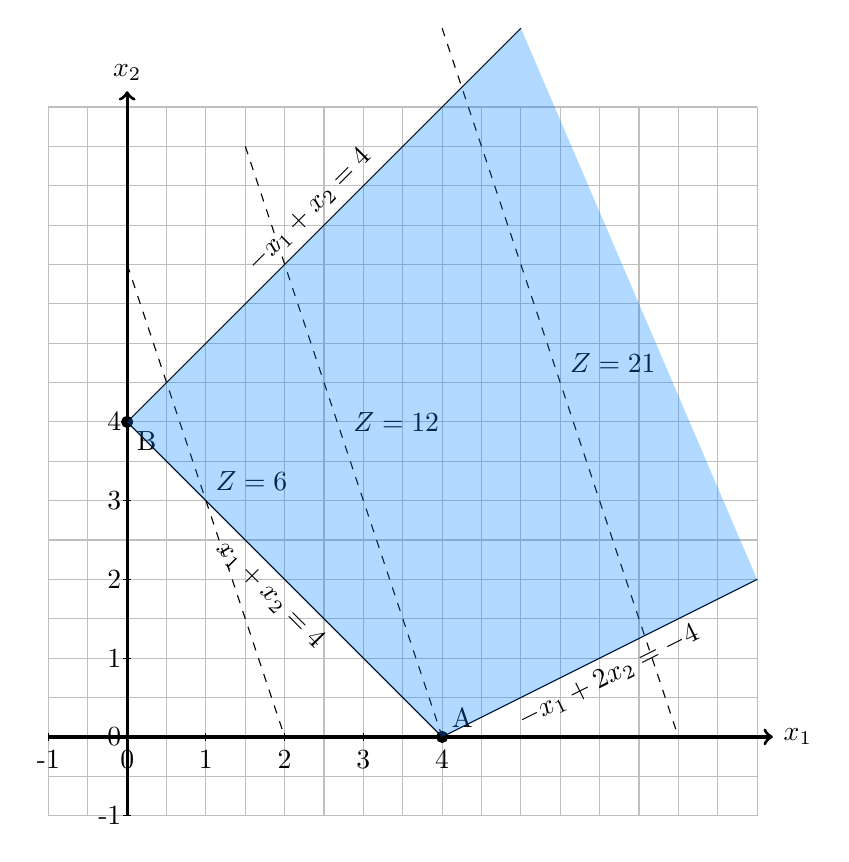
\begin{tikzpicture}

    \draw[gray!50, thin, step=0.5] (-1,-1) grid (8,8);
    \draw[very thick,->] (-1,0) -- (8.2,0) node[right] {$x_1$};
    \draw[very thick,->] (0,-1) -- (0,8.2) node[above] {$x_2$};

    \foreach \x in {-1,...,4} \draw (\x,0.05) -- (\x,-0.05) node[below] {\x};
    \foreach \y in {-1,...,4} \draw (-0.05,\y) -- (0.05,\y) node[left] {\y};

    \draw (0,4) -- node[above,sloped] {$-x_1+x_2=4$}  (5,9);
    \draw (0,4) -- node[below, sloped] {$x_1+x_2=4$} (4,0);
    \draw (4,0) -- node[below,sloped] {$-x_1+2x_2=-4$} (8,2);
    \draw[dashed] (0,6) -- node[above right] {$Z=6$} (2,0);
    \draw[dashed] (1.5,7.5) -- node[above right] {$Z=12$} (4,0);
    \draw[dashed] (4,9) -- node[above right] {$Z=21$} (7,0);

    \filldraw [black] (4,0) circle (2pt) node[above right] {A};
    \filldraw [black] (0,4) circle (2pt) node[below right] {B};

    \fill[blue!50!cyan,opacity=0.3] (0,4) -- (5,9) -- (8,2) -- (4,0) -- (0,4);

\end{tikzpicture}

\end{document}
